\section{Introduction}
\label{sec:introduction}
% state the learning objective 
The objective of this laboratory assignment is to study the behaviour of an RC circuit, as seen in Figure~\ref{fig:rc}. In order to analyse it, we will make use of different techniques such as Thevenin and Phasor analysis in order to establish the natural, forced and total solutions of the circuit. A frequency response analysis then follows, where we look at the magnitude and phase as a function of frequency. Then, we compare the theoretical and simulation data.

In Section~\ref{sec:analysis}, we go through the various steps that are needed to obtain the total solution of the circuit (natural plus forced responses) and present the theoretical frequency response analysis.
In Section~\ref{sec:simulation}, we present the circuit response as simulated in NGSpice. The results in operating point and transient analysis are compared to the theoretical results obtained in Section~\ref{sec:analysis}. The conclusions of this study are laid out in
Section~\ref{sec:conclusion}.

\begin{figure}[h] \centering
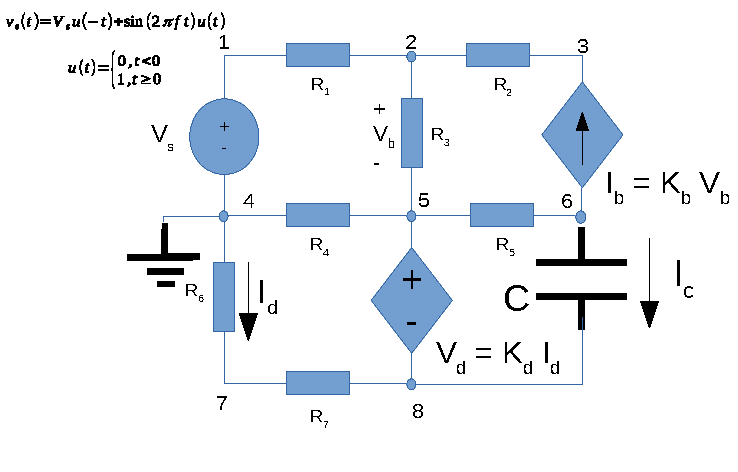
\includegraphics[width=0.9\linewidth]{rc.pdf}
\caption{RC circuit.}
\label{fig:rc}
\end{figure}

